\documentclass[a4paper, 11pt]{article}
\usepackage{fullpage} % changes the margin
\usepackage{url} % enable urls in document
\usepackage{ntheorem}
\usepackage{graphicx}
\usepackage{subcaption}
\usepackage[utf8]{inputenc}
\theoremseparator{:}
\newtheorem{hyp}{Hypothese}

\newcommand{\projectName}{mci-af}
% Ideen für Namen: 
%   Koala [weil sie fucking lange schlafen (22h)]
%   Resync [kurz für resynchronization, also das 'in-Einklang-bringen' von dem, was das System weiß und dem, was der Benutzer weiß]
%   TAIN [TAsk INertia - Aufgaben Trägheit]

\begin{document}
\begin{center}
	\textbf{\LARGE{\projectName}}\\
    \textbf{\large{Anwendungsfach Mensch Computer Interaktion}}\\
	\vspace{7mm}
    \textbf{\large{Böhm, Sabrina; Porta, Luca; Lahmann, Tobias}}\\
	\textbf{\large{Betreuer: Dennis Wolf}}\\
	\today
\end{center}

\section*{Abstract}
Die Untersuchung der Heranführung einer Person an ein Problem, wenn diese im vorfeld keine Informationen über die Aufgabe hat. % Introduction. In one sentence, what’s the topic?
Wir untersuchen die unterschiedlichen Arten jemanden aus einem trance-ähnlichen Zustand, wie sie nach dem Schlafen auftreten kann, in einen Bewussten zu überführen und wie diese Person in diesem Vorgang unterstützt werden kann. % State the problem you tackle
Vorbereitungen auf Aufgaben und noch spezieller die Lenkung der Aufmerksamkeit bei dieser wurde noch ungenügend untersucht. % Summarize (in one sentence) why nobody else has adequately answered the research question yet
Wir untersuchen die Problemstellung im Kontext von VR und nutzen dies um dadurch unterschiedliche Parameter des 'Aufweckens' sowie Designprinzipien zu untersuchen. % Explain, in one sentence, how you tackled the research question
In einer between-subject Studie wurden die Unterschiede der möglichen Designs untersucht. % In one sentence, how did you go about doing the research that follows from your big idea
Aktuell können unsere Vermutungen noch nicht bestätigt werden. % As a single sentence, what’s the key impact of your research?

\section*{Motivation}
Virtuelle und Augmentierte Umgebungen begleiten uns bereits seit einigen Jahren. Diese Systeme benötigen aber immer ein Gerät zum Anzeigen der Inhalte, welches aktiv Aufgesetzt werden muss bzw. nicht permanent getragen werden kann. Werden in Zukunft diese Systeme kleiner, leichter, oder sogar permanent mit dem menschlichen Körper verbunden, wird es möglich jeden Bereich des Lebens zu augmentieren. In diesem Projekt möchten wir erforschen inwieweit die Systeme den Nutzer auf unerwartete Aufgaben vorbereiten können. So können in autonomen Autos Aufgaben vom Fahrer übernommen, im Nachtdienst eines Sicherheitsunternehmens kritische Vorgänge überwacht, oder am Morgen Herausforderungen vom Benutzer verlangt werden, welche ein hohes Maß an Aufmerksamkeit erfordern. Wir möchten herausfinden wie schnell und effizient ein Benutzer auf diese Aufgaben Vorbereitet werden kann. -tl

\section*{Problemstellung}
In unterschiedlichsten Fällen können Nutzer auf die Erledigung einer Aufgabe in einer virtuellen Umgebung nur schwer vorbereitet werden, wenn diese  plötzlich oder ohne Überleitung gestellt wird. So können Nutzern einer virtuellen oder augmentierten Realität (VR/AR) beim Wechsel der Umgebung, oder beim Wechsel in die digitale Umgebung, Informationen fehlen, welche notwendig sind um sich schnell, zuverlässig und ohne potenzielle Fehlerquellen an diese zu gewöhnen. 

Das Projekt "\projectName" soll es einem Nutzer ermöglichen alle relevanten Informationen innerhalb kürzester Zeit aufzunehmen. Des Weiteren soll untersucht werden auf welche Art und Weise dieser Vorgang zuverlässig durchgeführt werden kann.

\section*{Verwandte Forschung}
Räumliche, aufmerksamkeitssensitive Darstellungen sind effektiv~\cite{bonanni2005attention}. Exogene Hinweise können dem Nutzer helfen sich auch in unbekannten Umgebungen zurechtzufinden~\cite{bonanni2005attention}.

Es existieren unterschiedliche Herangehensweisen um Fahrer in Autos über eine auftretende Gefahrensituation zu informieren. Hierbei wurden textuelle Informationen den grafischen vorgezogen.~\cite{green1995hazard}

Kulturelle Unterschiede bewirken, dass sich Fahrer im Straßenverkehr auf unterschiedliche Dinge konzentrieren und im Anschluss an unterschiedliche Details erinnern~\cite{yumiko2017VisAttention}.

Zur Vorbereitung auf die Objekte oder Vorgänge in der Umgebung von Menschen können 3D Marker verwendet werden, die in die Richtung des Objekts oder Geschehens weisen. Eine 3D Darstellung ist nach Chittaro und Burigat mindestens genauso effektiv wie eine 2D Darstellung. Sie bietet jedoch den Vorteil, dass Nutzer auch in der dritten Dimension, der Höhe, auf wichtige Punkte hingewiesen werden können~\cite{chittaro20043d}.

Schlafentzug verursacht tiefere Kurzschlaf-Phasen~\cite{dinges1985assessing}. Sollte eine optimale Performance in Aufgaben benötigt werden sollten Kurzschlaf-Phasen vermieden werden~\cite{dinges1985assessing}. Schlummern sowie Nickerchen sollten gemacht werden bevor ein gravierender Schlafentzug eintritt~\cite{dinges1985assessing}.

Abhängig von der Tageszeit existieren Unterschiede in der Performance, so wie der Selbsteinschätzung und anderer psychologischer Parameter bei voll ausgeschlafenen Probanden (12 Stunden Schlaf)~\cite{kraemer2000time}.

\section*{Lösungsansatz}
In einer virtuellen Umgebung werden Probanden dazu aufgefordert sich zu entspannen und, nach Möglichkeit, ohne Ablenkung zu verweilen. Das Ziel ist es den Nutzer in einen Zustand der Trägheit zu versetzten, wie er nach dem Schlafen auftreten kann. In diesem Zustand könnten Informationen nur schwer aufgenommen werden und eine Aufgabe, die in diesem Zeitraum gestellt wird könnte so mit geringerem Erfolg erledigt werden, als wenn der Nutzer voll aufnahmefähig ist. 

Im Anschluss an die initiale Ruhephase werden die Nutzer auf unterschiedliche Arten `auf\-geweckt' und ihnen wird eine oder mehrere Aufgaben gestellt. Eine Gruppe der Nutzer wird `sanft geweckt' indem die virtuelle Umgebung langsam und bedacht erhellt wird, zudem kann dieser Vorgang mit unterschiedlichen anderen Sinnen unterstützt werden. Die Aufgabenstellung erscheint iterativ und wird mit jedem Schritt anspruchsvoller, bis die volle Schwierigkeit erreicht wurde. 
Die andere Gruppe der Nutzer wird hingegen `schnell geweckt'. Hierbei wird die Helligkeit der Virtuellen Umgebung plötzlich erhöht. Auch hier können unterschiedliche Sinne angesprochen werden um möglicherweise den Stressfaktor beim Probanden zu erhöhen. Die Nutzer werden direkt nach dem Aufwachen mit der vollen Schwierigkeit einer Aufgabe konfrontiert und müssen diese lösen.

Im nächsten Schritt des Projekts soll untersucht werden auf welche Arten die Nutzer der beiden Gruppen in dem Erledigen von Aufgaben unterstützt werden können. Hierbei werden vor allem gestalterische sowie aufmerksamkeitssteuernde Aspekte untersucht. 

Die Nutzer beider Gruppen können hier dahingehend untersucht werden, mit welchen Fehlerraten sowie welcher Geschwindigkeit die gestellten Aufgaben erledigt werden. Nachfolgend können standardisierte Fragebögen herangezogen werden um das Befinden und die Einschätzung des Nutzers zu untersuchen.

Eye-Tracking wird verwendet, um zu untersuchen in welchem Müdigkeit-Stadium sich die Probanden befinden.

Wir stellen grundlegend die folgenden Hypothesen auf:
\begin{hyp}[H\ref{hyp:schneller}]\label{hyp:schneller}
	Menschen die langsam geweckt werden können sich in kürzerer Zeit auf eine gestellte Aufgabe einstellen, als Menschen, die abrupt aus dem Schlaf gerissen werden.
\end{hyp}

\begin{hyp}[H\ref{hyp:erfolgreicher}]\label{hyp:erfolgreicher}
	Menschen die langsam geweckt werden können eine gestellte Aufgabe mit weniger Fehlern erledigen, als Menschen, die abrupt aus dem Schlaf gerissen werden.
\end{hyp}

und

\begin{hyp}[H\ref{hyp:gestaltung}]\label{hyp:gestaltung}
    Prozedurale Informationen (4C-ID)~\cite{van2002blueprints} bewirken, dass Benutzer eine Aufgabe schneller, sowie mit einer geringeren Fehlerrate erledigen können.
\end{hyp}

\section*{Implementierung}
Auf Softwareseite soll eine digitale Umgebung mittels Unity 3D\footnote{~Unity3D~\url{https://unity3d.com}} erstellt werden. Das gewählte Interface zur Untersuchung der beschriebenen Problemstellung ist die HTC Vive\footnote{~HTC Vive~\url{https://www.vive.com}} mit den zugehörigen Controllern. Bewegung innerhalb der digitalen Umgebung ist, bis auf Kopfbewegungen, nicht vorgesehen, da die Probanden in einem sitzenden Zustand untersucht werden. Die Eingabemethoden zur Bewältigung der gestellten Aufgaben werden mit Zeigeoperationen innerhalb der virtuellen Umgebung realisiert. Eine Implementierung zum Nachverfolgen der Augenbewegung von Probanden (Eye-Tracking) wird nicht selbst durchgeführt, sondern auf bestehende Implementierungen zurückgegriffen. 

Fragebögen werden über das Limesurvey online Fragebogen Tool der Universität Ulm\footnote{~Limesurvey~\url{https://surveys.informatik.uni-ulm.de/limesurvey/
}} gestellt und beantwortet. 

\subsubsection*{Aufwachen}
Probanden können auf unterschiedliche Arten aufgeweckt werden
\begin{itemize}
    \item \textbf{Töne} Alarm-Sounds oder Musik~[cite needed]
    \item \textbf{Licht} Helle Umgebungen wecken Personen auf~[cite needed]
    \item \textbf{Temperatur} Eine kalte Umgebung verursacht erhöhte Aufmerksamkeit~[cite needed]
    \item \textbf{Bewegung} Jemand der geschüttelt wird wacht ebenfalls auf~[cite needed]
\end{itemize}

\section*{Testaufbau}
Sitzend werden Probanden erst in einen entspannten Zustand versetzt. In diesem sollen sie möglichst ohne Ablenkung verweilen bis sich eine Gelassenheit oder Trägheit einstellt. Diese kann von entspanntem Sitzen bis hin zum Schlaf führen, eine genaue Zeitspanne hierfür kann zwischen Probanden variieren und muss in Tests bestimmt werden.

Nachfolgend wird der Teilnehmer aus diesem Zustand geleitet und mit einer Aufgabe konfrontiert. Während der Erledigung dieser werden unterschiedliche Parameter (Blickrichtung, Zeit und Fehlerrate der Erledigung der Aufgabe) aufgezeichnet und später ausgewertet.

\subsubsection*{Aufgaben}
Die folgenden Aufgaben können implementiert werden um den Nutzer zu beschäftigen und seine Leistungsfähigkeit zu ermitteln:
\begin{enumerate}
    \item \textbf{Stroop-Effekt} Im Mittelpunkt des Blickfeldes wird eine ausgeschriebene Farbe angezeigt. Die Textfarbe des Worts muss nicht zwangsläufig die der ausgeschriebenen Farbe sein. Der Proband soll als Eingabe die Textfarbe auswählen indem er mit dem Controller auf einem Interface die richtige Auswahl trifft. Beispiel kann in Figure~\ref{fig:stroop_test} gesehen werden.
    \item \textbf{Zahlenfolge} Verteilt über das Blickfeld des Probanden werden Zahlen angezeigt. Die Abstände zwischen den Zahlen sind nicht gleichverteilt und werden idealerweise so gewählt, dass eine Verwechslungsgefahr besteht. Aufsteigend sollen die Zahlen selektiert und so geordnet werden. (123 $\rightarrow$ 324 $\rightarrow$ 823 $\rightarrow$ 1237 ...)
    \item \textbf{Senso / Simon} Nach vorlage des bekannten Spiels werden Sequenzen auf einer 4-Felder-Farbmatrix vorgegeben, die vom Probanden wiederholt werden müssen. Beispiel kann in Figure~\ref{fig:simon} gesehen werden.
\end{enumerate}

\begin{figure}
	\centering
	\begin{subfigure}{0.4\textwidth} % width of left subfigure
		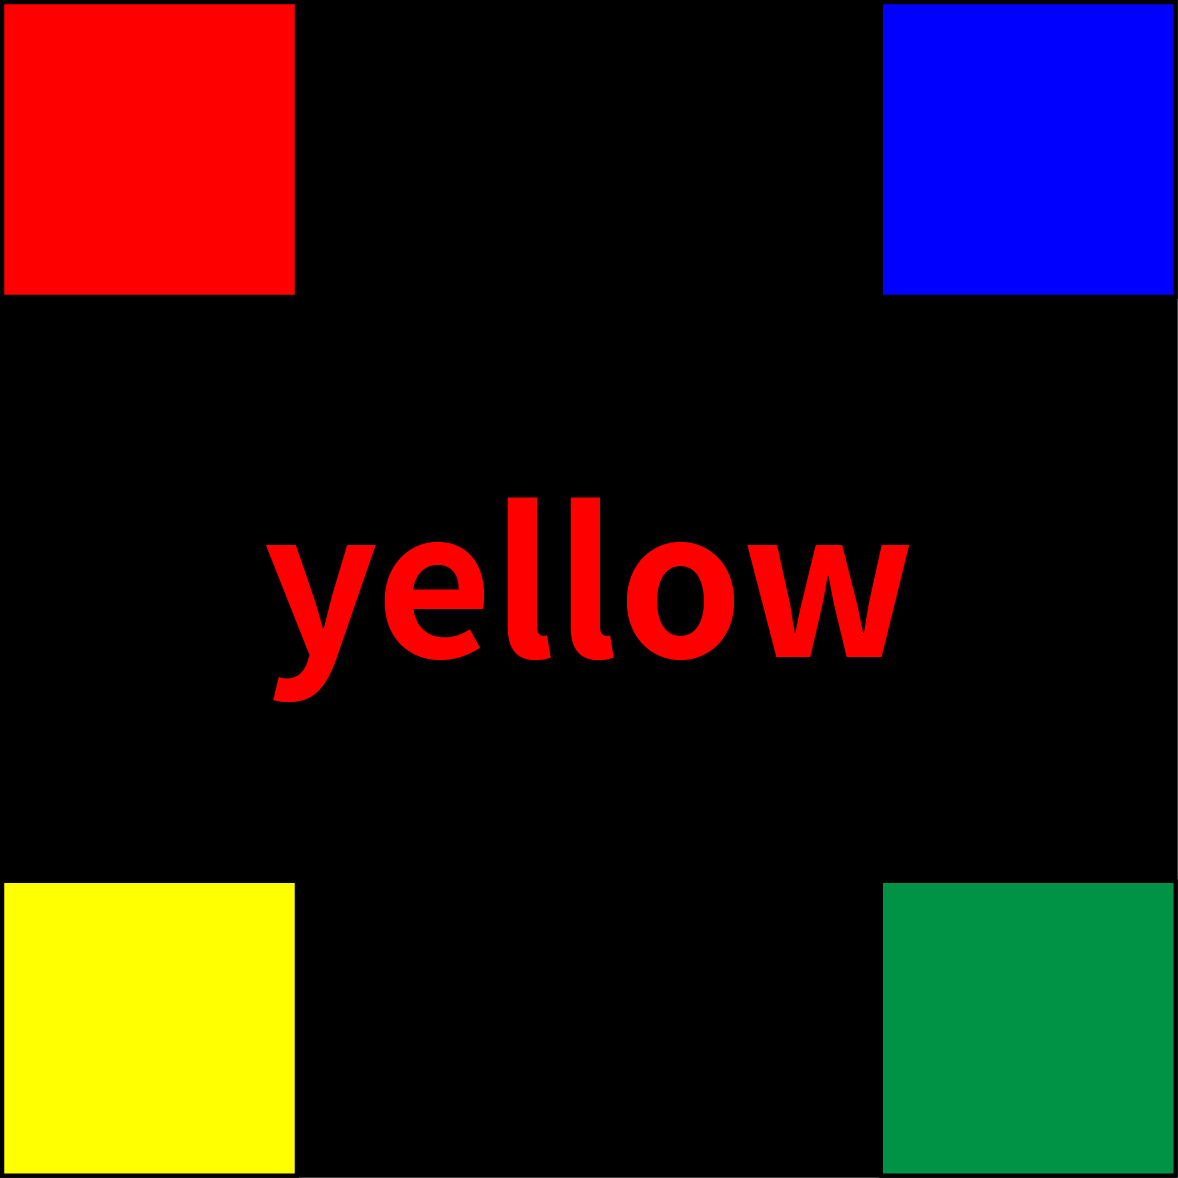
\includegraphics[width=\textwidth]{./figures/Reversed_stroop_test.jpg}
        \caption{Stroop Test, ElvisLin CC BY-SA 4.0. \url{https://commons.wikimedia.org/wiki/File:Reversed_stroop_test.jpg}} % subcaption
        \label{fig:stroop_test}
	\end{subfigure}
	\vspace{1em} % here you can insert horizontal or vertical space
	\begin{subfigure}{0.534\textwidth} % width of right subfigure
		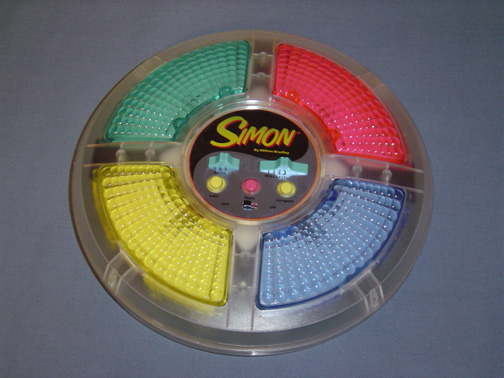
\includegraphics[width=\textwidth]{./figures/Simon_game.jpg}
		\caption{Senso / Simon, Larry D. Moore CC BY-SA 3.0. \url{https://commons.wikimedia.org/wiki/File:Simon_game.jpg}} % subcaption
        \label{fig:simon}
	\end{subfigure}
	\caption{Beispiele für die Spiele mit denen die Teilnehmer konfrontiert werden.} % caption for whole figure
\end{figure}

\section*{Zeitplan}
Die Daten beziehen sich auf den Zeitpunkt zu dem der jeweilige Schritt abgeschlossen sein sollte.
\begin{itemize}
    \item \textbf{Dezember 2018} Recherche bestehender Forschung
    \item \textbf{Dezember 2018} Digitale Umgebung in Unity3D erstellen und mit erster Testphase validieren
    \item \textbf{Dezember 2018} Erste Studie durchführen
    \item \textbf{Januar 2019} Auswertung der durchgeführten Studie.
    \item \textbf{März 2019} Entwurf der zweiten Studie
    \item \textbf{April 2019} Erweiterte Umgebung in Unity3D erstellen und für den zweiten Studiendurchlauf vorbereiten
    \item \textbf{Mai 2019} Durchführung der zweiten Studie für erweiterte Ergebnisse
    \item \textbf{Juni 2019} Auswertung der Ergebnisse von zweiter Studie
    \item \textbf{September 2019} Dokumentation der Ergebnisse und des Vorgehens
\end{itemize}

\begin{thebibliography}{9}
\bibitem{yumiko2017VisAttention} Shinohara, Yumiko, et al. "Visual Attention During Simulated Autonomous Driving in the US and Japan." Proceedings of the 9th International Conference on Automotive User Interfaces and Interactive Vehicular Applications. ACM, 2017.
\bibitem{bonanni2005attention} Bonanni, Leonardo, Chia-Hsun Lee, and Ted Selker. "Attention-based design of augmented reality interfaces." CHI'05 extended abstracts on Human factors in computing systems. ACM, 2005.
\bibitem{green1995hazard} Green, Paul. "A driver interface for a road hazard warning system: Development and preliminary evaluation." Proceedings of the Second World Congress on Intelligent Transportation Systems. Vol. 4. 1995.
\bibitem{chittaro20043d} Chittaro, Luca, and Stefano Burigat. "3D location-pointing as a navigation aid in Virtual Environments." Proceedings of the working conference on Advanced visual interfaces. ACM, 2004.
\bibitem{wilkinson1971performance} Wilkinson, Robert T., and M. Stretton. "Performance after awakening at different times of night." Psychonomic Science 23.4 (1971): 283-285.
\bibitem{dinges1985assessing} Dinges, David F., Martin T. Orne, and Emily Carota Orne. "Assessing performance upon abrupt awakening from naps during quasi-continuous operations." Behavior research methods, instruments, \& computers 17.1 (1985): 37-45.
\bibitem{kraemer2000time} Kraemer, Susanne, et al. "Time-of-day variations of indicators of attention: performance, physiologic parameters, and self-assessment of sleepiness." Biological psychiatry 48.11 (2000): 1069-1080.
\bibitem{van2002blueprints} Van Merriënboer, Jeroen JG, Richard E. Clark, and Marcel BM De Croock. "Blueprints for complex learning: The 4C/ID-model." Educational technology research and development 50.2 (2002): 39-61.
\end{thebibliography}

\listoffigures	% Abbildungsverzeichnis

\end{document}
